
\lhead[\chaptername~\thechapter]{\rightmark}


\rhead[\leftmark]{}


\lfoot[\thepage]{}


\cfoot{}


\rfoot[]{\thepage}


\chapter{Ergebnisse und Diskussion}

\begin{figure}
	\centering
	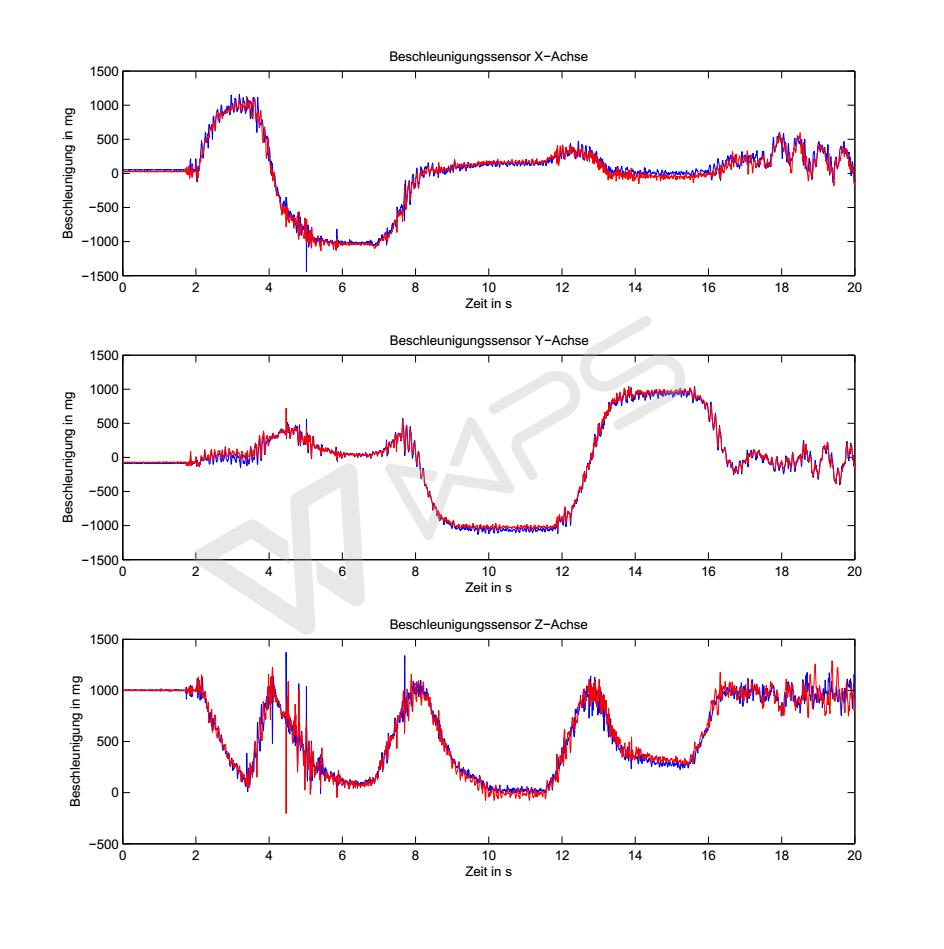
\includegraphics[width=1\textwidth]{images/Messergebnisse/calibration-wood-accel111}
	\caption{Kalibrierung mit Holzgestell, Beschleunigungssensor.}
\end{figure}

\begin{figure}
	\centering
	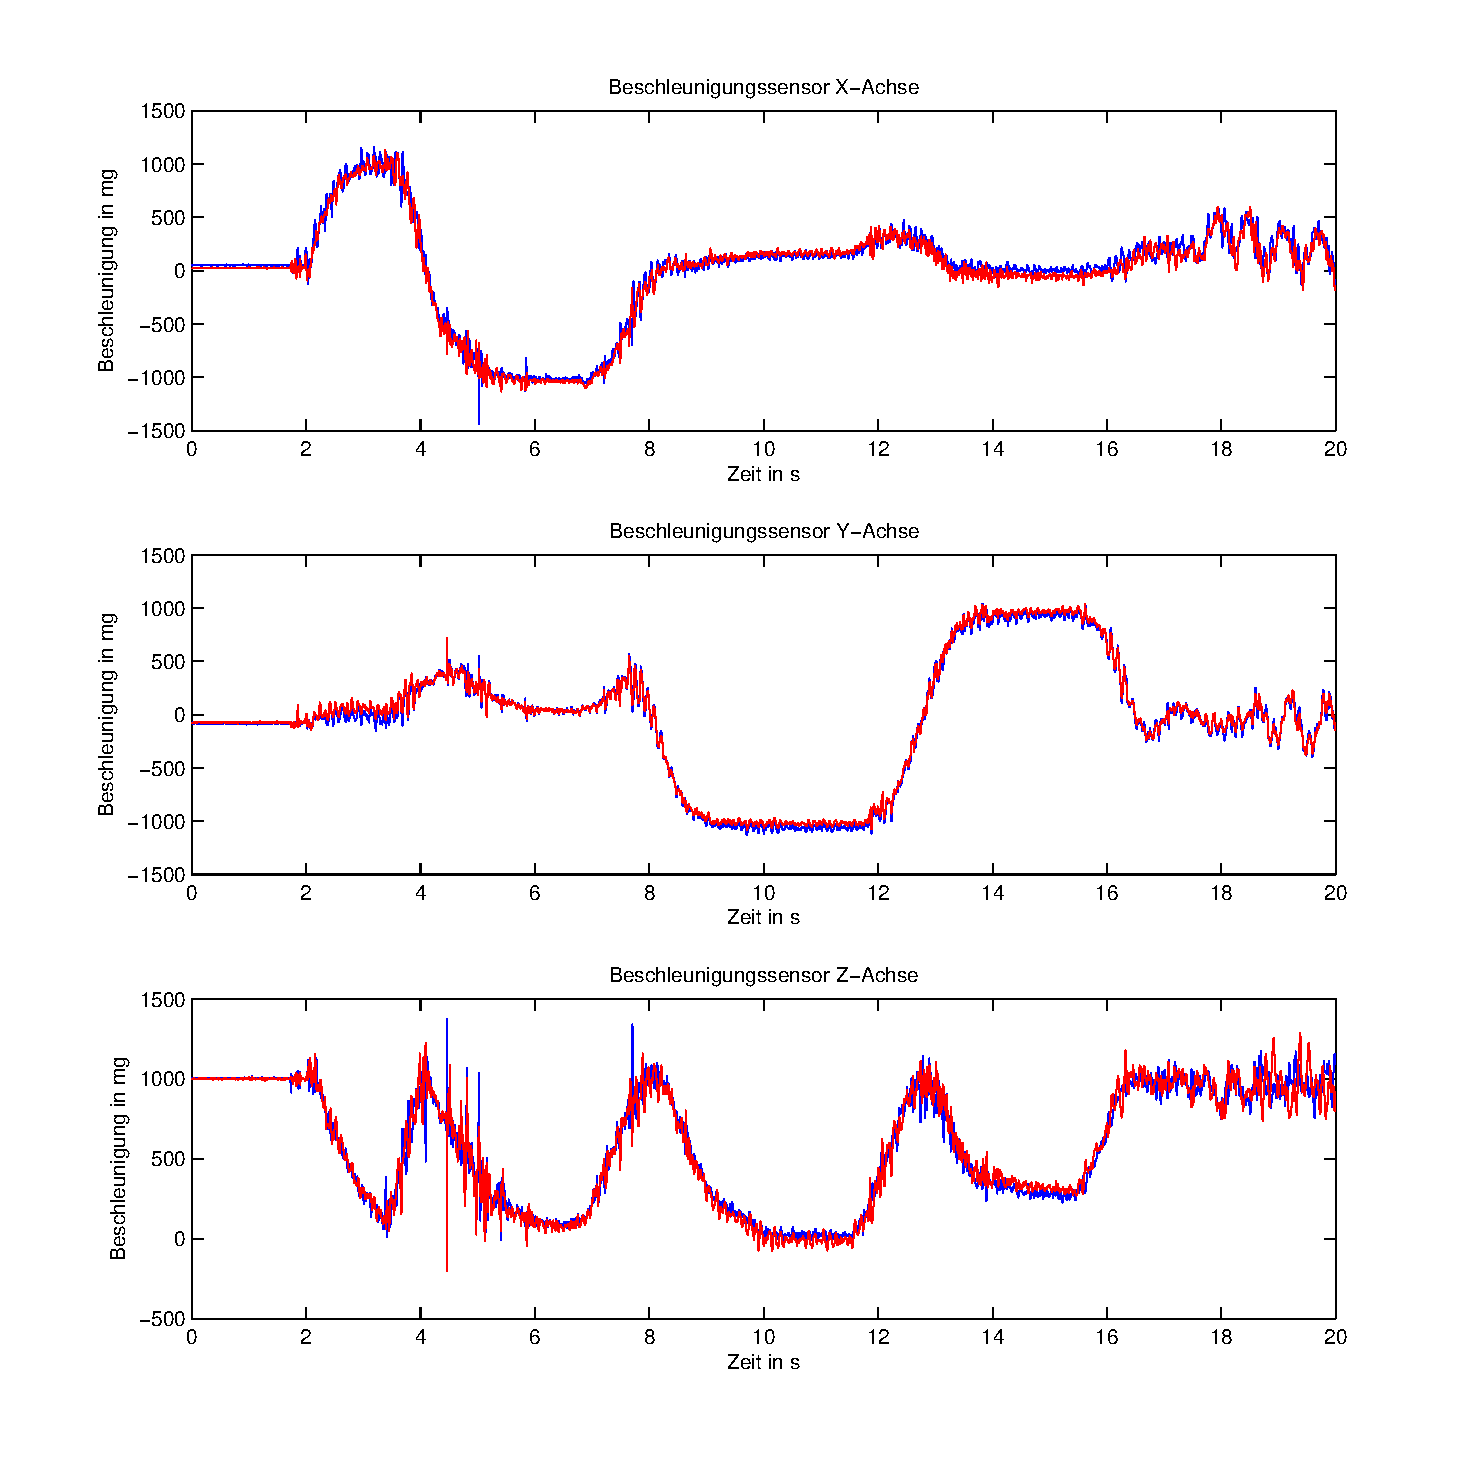
\includegraphics[width=1\textwidth]{images/Messergebnisse/calibration-wood-accel}
	\caption{Kalibrierung mit Holzgestell, Beschleunigungssensor.}
\end{figure}










